\chapter{Finite Element Modeling}
\label{ch:nastran}

An existing finite element model (FEM) of MARGE was updated in this study using NASTRAN. The model included MARGE, the wind tunnel test section walls, and the gust vanes. This chapter describes the FEM; the updates applied to it are documented in Chapter \ref{ch:gvt}.

The wing structure and tail structure were each modeled as a single chain of Euler-Bernoulli beam elements along their respective spar. The wind tunnel walls were modeled as extremely rigid panels whose contribution to the structural dynamics of the FEM is negligible. The area moments of inertia and material properties of the beam elements in the finite element model are reported in Table \ref{tab:beamInertia}.
\begin{table}[H]
    \centering
    \caption{Properties of Beam Finite Elements}
    \label{tab:beamInertia}
    \begin{tabular}{lccccc}
        \hline\hline
                  & $E$, GPa & $G$, GPa & $I_1$, mm$^4$ & $I_2$, mm$^4$ & $J$, mm$^4$ \\
        \hline
        wing spar & $68.9$   & $0.0125$ & $25.41$       & $58530$       & $58560$     \\
        tail spar & $68.9$   & $25.9$   & $1829$        & $13010$       & $14840$     \\
        fuselage  & $200$    & $76.0$   & $74.52$       & $4476 $       & $4550 $     \\
        rigid     & $10^4$   & $10^4$   & $25.41$       & $58530$       & $58560$     \\
        \hline\hline
    \end{tabular}
\end{table}
Note that the values in Table \ref{tab:beamInertia} (and also Table \ref{tab:nastranResult}) are the final values after corrections. The values before corrections and correction process are discussed in the following chapter.

The aerodynamic loads on the NASTRAN model are based on the doublet-lattice model (DLM) for aerodynamics. This linear aerodynamic model assumes incompressible, inviscid, irrotational flow around thin lifting surfaces. The loads on the aerodynamic panels were transferred to the structural nodes via a spline interpolation. The aerodynamic panels and structural finite elements can be seen in Fig. \ref{fig:nastranWindowFull}. Figure \ref{fig:nastranWindowClose} shows a close-up view of MARGE in the FEM. Details of the implementations and limitations of these theories can be found in the NASTRAN Aeroelastic Analysis User's Guide \cite{Siemens2020}

The structural dynamic solution to the FEM includes natural frequencies and mode shapes. These are summarized in Table \ref{tab:nastranResult}.
\begin{table}[H]
	\centering
	\caption{NASTRAN Modal Properties}
	\label{tab:nastranResult}
	\begin{tabular}{cll}
		\hline\hline
		\# & $\omega_n$ & Description \\
		\hline
		1  &   0     & pitching \\
		2  &   1.444 & wing bending 1 \\
		3  &  10.487 & wing bending 2 \\
		4  &  16.638 & fuselage bending 1 \\
		5  &  19.200 & wing twisting 1 \\
		6  &  21.948 & fuselage in-plane bending 1 \\
		7  &  32.311 & wing bending 3 \\
		8  &  60.852 & fuselage bending 2 \\
		9  &  66.011 & wing bending 4 \\
		10 &  69.298 & wing in-plane bending 1 \\
		11 & 113.674 & wing bending 5 \\
		12 & 120.642 & fuselage bending 3 \\
		13 & 153.716 & fuselage in-plane bending 2  \\
		14 & 160.909 & fuselage bending 4 \\
		15 & 175.941 & wing bending 6 \\
		\hline\hline
	\end{tabular}
\end{table}

% HERE BE THE NASTRAN SCREENSHOTS

\begin{landscape}

\begin{figure}[h]
	\centering
	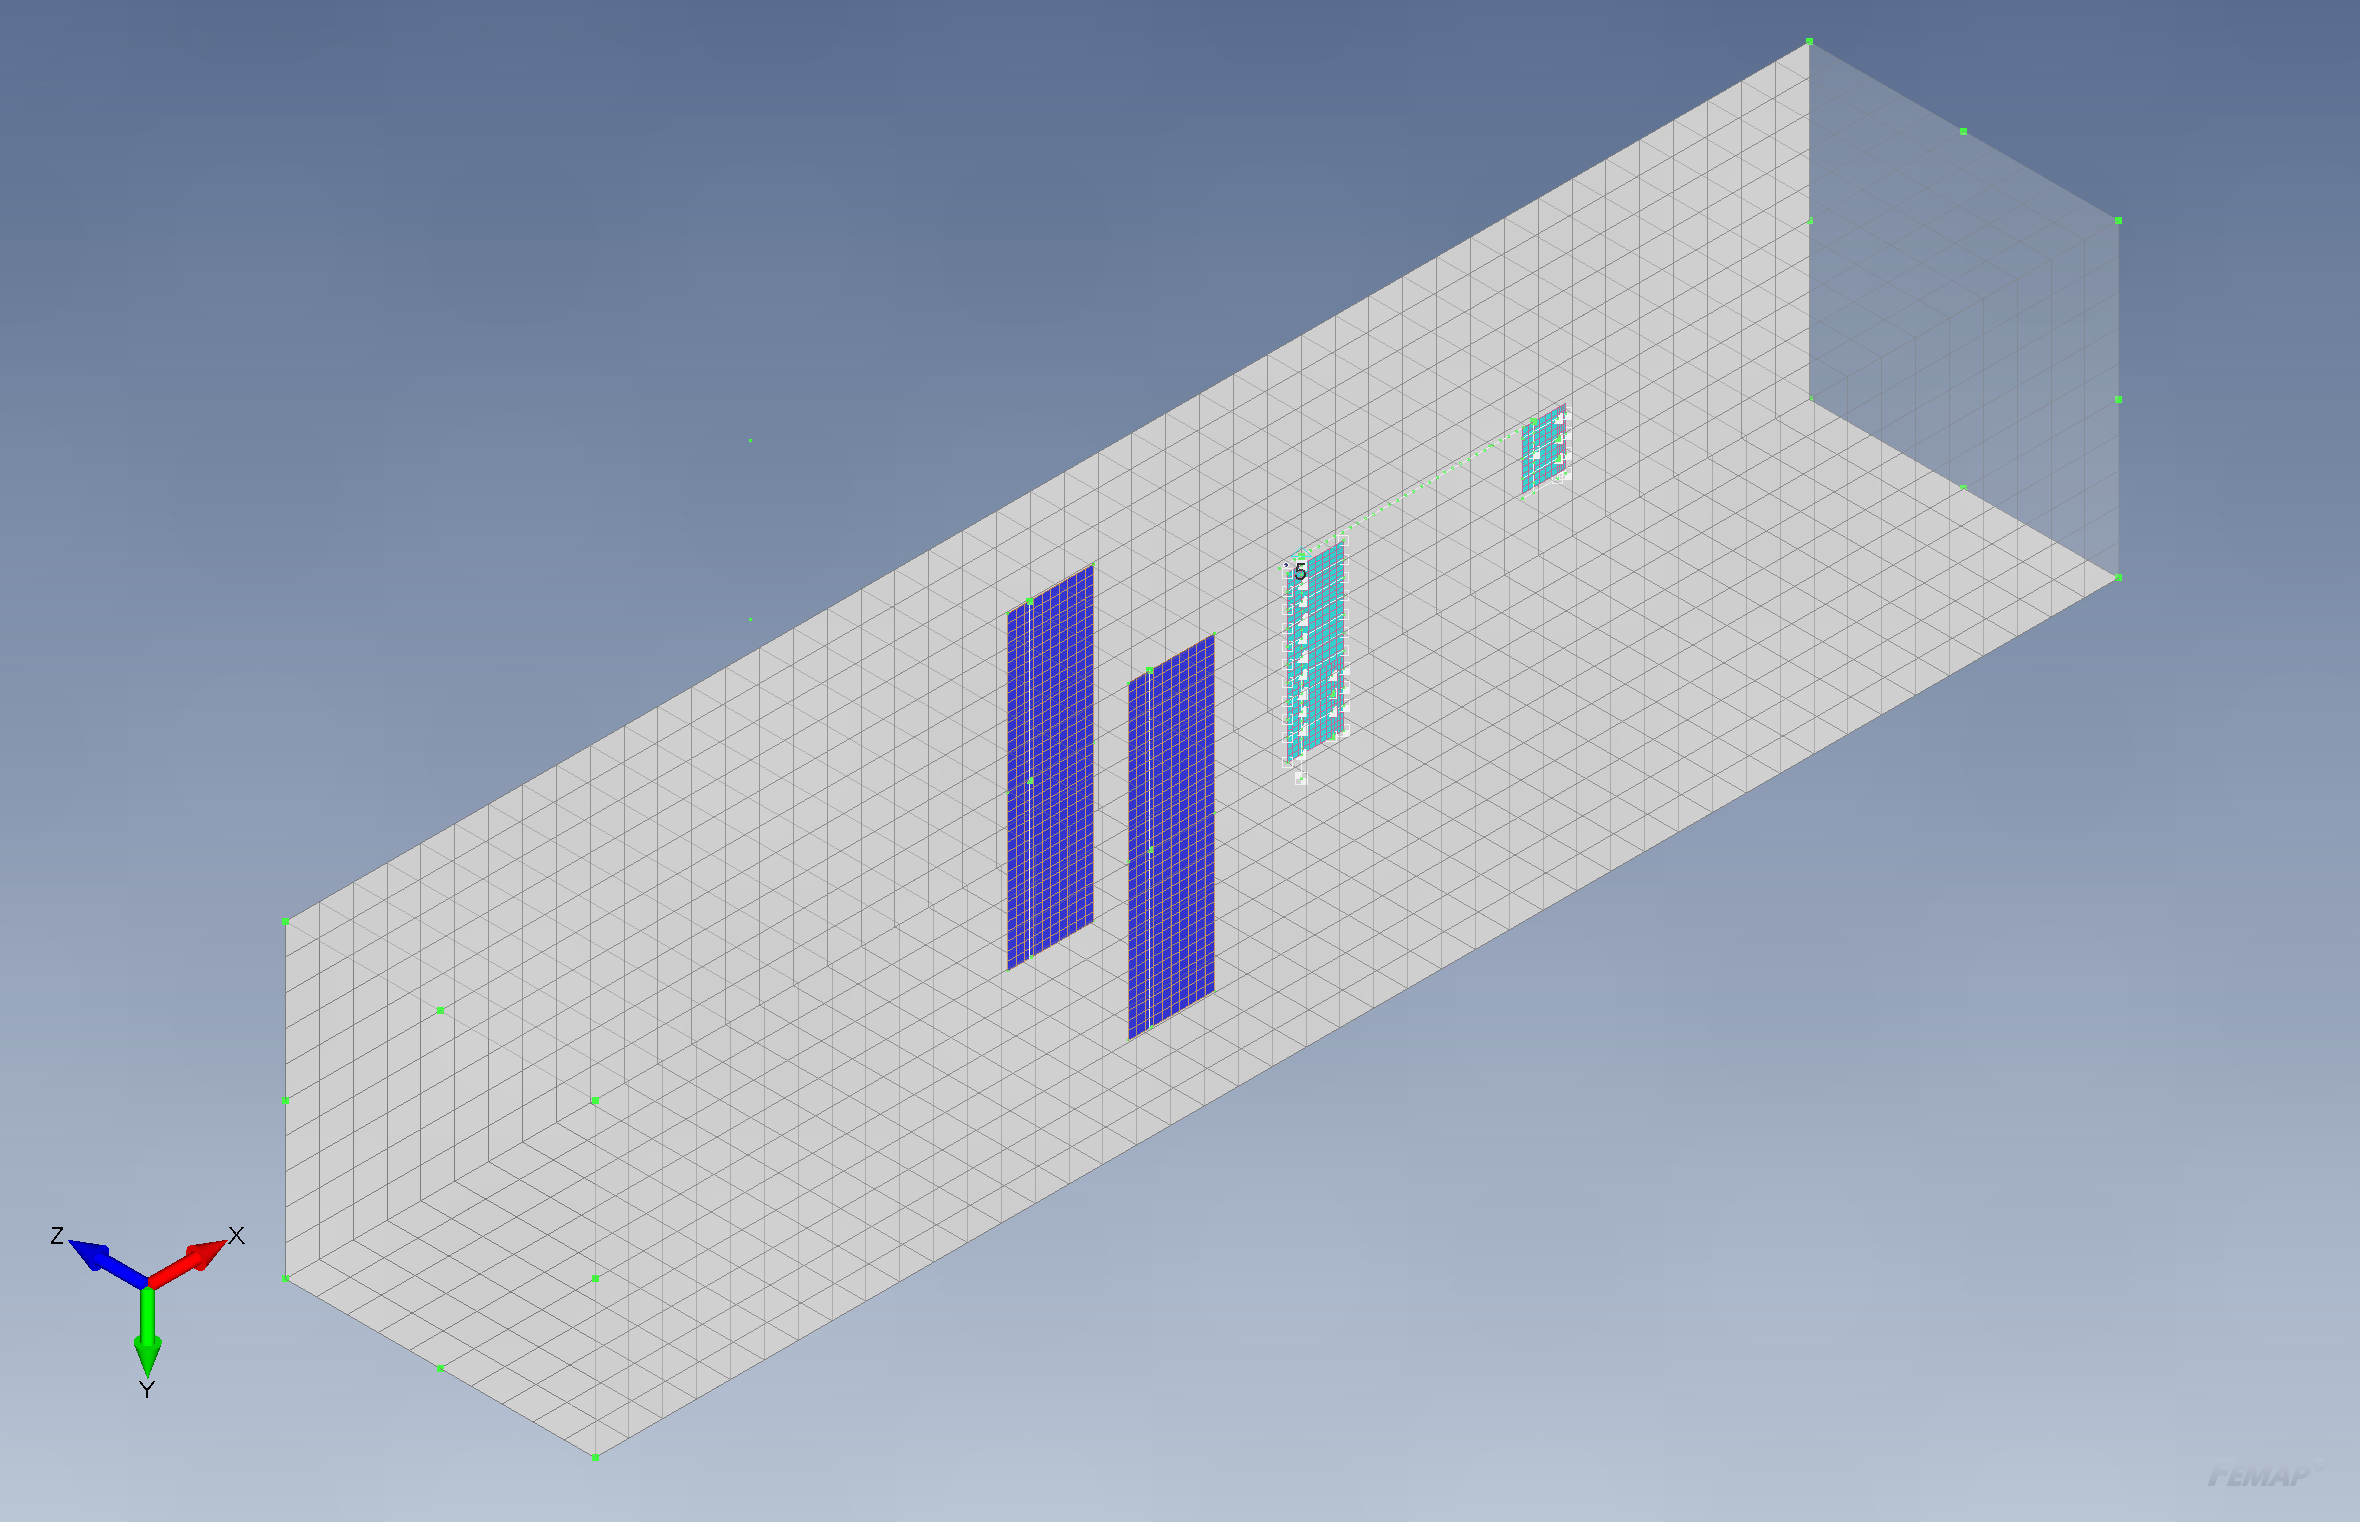
\includegraphics[width=9in]{margeFEMfull.png}
	\caption{NASTRAN finite-element model of MARGE, gust vanes, and wind tunnel walls}
	\label{fig:nastranWindowFull}
\end{figure}
\begin{figure}[h]
	\centering
	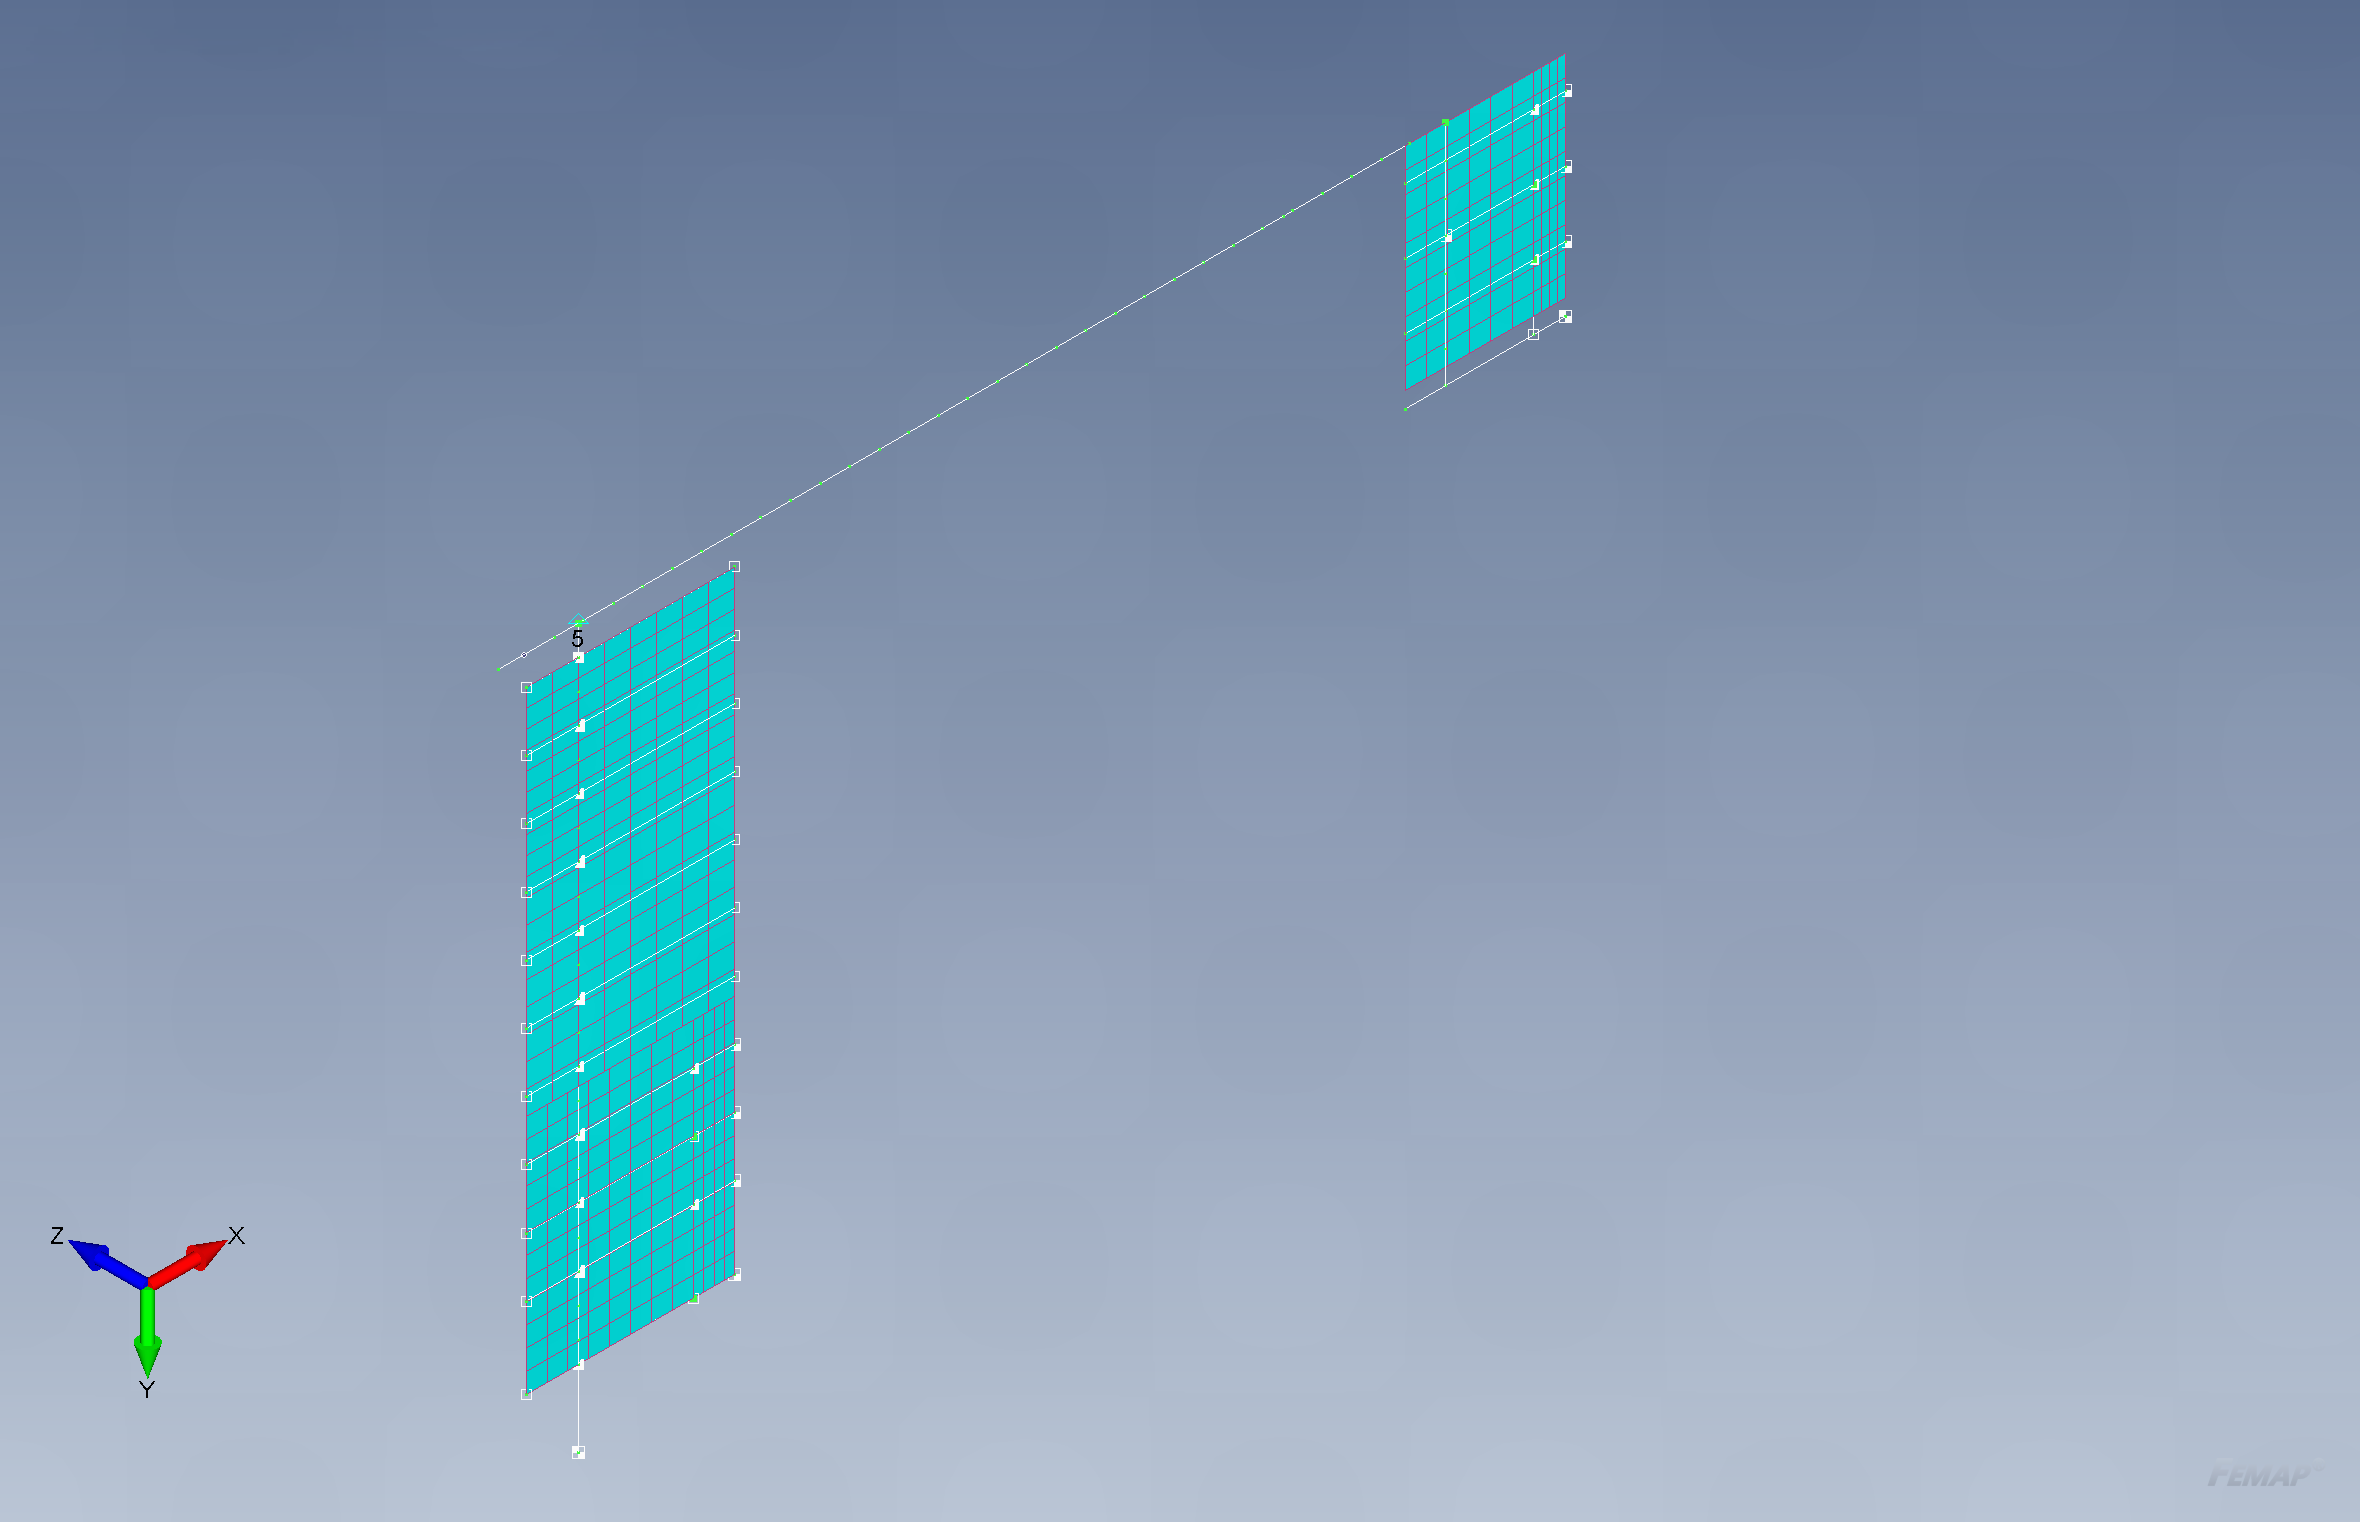
\includegraphics[width=9in]{margeFEMclose.png}
	\caption{NASTRAN finite-element model, close-up of MARGE only}
	\label{fig:nastranWindowClose}
\end{figure}

\end{landscape}